\documentclass[utf8, seminar, numeric, lmodern]{feri}

\renewcommand{\familydefault}{\sfdefault}	% sans-serif main
%\usepackage{inconsolata}					% sans-serif monospace
\usepackage[scaled]{beramono}				% sans-serif monospace

\raggedright						% bez desnog poravnavanja
\usepackage{caption}
\captionsetup{%
	justification=raggedright,
}
\setlength{\parindent}{1em}			% uvlačenje ulomaka
\usepackage{indentfirst}			% uvlačenje prvog ulomka
\setlength{\parskip}{0.5em}			% razmak između ulomaka

\usepackage[T1]{fontenc}  % accented characters, copy from pdf, ...

\usepackage{listings}					% listings
\renewcommand{\lstlistingname}{Ispis}
%\usepackage{floatrow} 				% centriranje svih slika
\usepackage{float}					% figure [H]
\usepackage{graphicx} 				% includegraphics
	\usepackage{caption}			% subfigure
	\usepackage{subcaption}			% subfigure
	\usepackage[export]{adjustbox} 	% http://ctan.org/pkg/adjustbox
	\graphicspath{ {./ilustracije/} }		% mapa sa slikama
	\let\oldincludegraphics\includegraphics
	\renewcommand{\includegraphics}[2][]{\oldincludegraphics[#1,max width=0.9\linewidth]{#2}}
\usepackage{tikz} 					% dijagrami
  \tikzset{>=latex}
  \usepackage{pgfplots}
	  \pgfplotsset{every axis/.append style={
	  		axis x line=middle,    	% put the x axis in the middle
	  		axis y line=middle,    	% put the y axis in the middle
	  		axis line style={->},  	% arrows on the axis
	  		xlabel={$x$},          	% default put x on x-axis
	  		ylabel={$y$},          	% default put y on y-axis
	  		samples=100,
	  		axis equal,
	  	}} % axis style
	\usetikzlibrary{fit}
	
\usetikzlibrary{automata,arrows,positioning,calc}
\usetikzlibrary{arrows,%
	petri,%
	topaths}%
	
\usepackage[croatian]{babel}		% teorem

\usepackage{amsmath}

\usepackage{commath}  % abs, norm, derivacije (\od[2]{f}{x}, \od[2]{f}{x} \dif x = dx)


\usepackage{bm}

%\newtheorem{definition}{Definicija}[section]
%\newtheorem{theorem}{Teorem}[section]
%\newtheorem{corollary}{Korolar}[theorem]

\DeclareMathOperator{\step}{step}
\DeclareMathOperator{\Heaviside}{H}
\DeclareMathOperator{\Ramp}{R}
\DeclareMathOperator{\softplus}{softplus}
\DeclareMathOperator{\softmax}{softmax}
\DeclareMathOperator{\logistic}{\sigma}

\newcommand{\mat}[1]{\bm{#1}}
%\newcommand{\m}[1]{\bm{#1}}
\let\vec\relax
\newcommand{\vec}[1]{\bm{#1}}
%\newcommand{\v}[1]{\bm{#1}}
\newcommand{\tens}[1]{\bm{\mathsf{#1}}} 	% undergraduate algebra version

\newcommand{\transpose}{\mathsf T} 	% undergraduate algebra version

\newcommand{\pderiv}[2]{\frac{\partial #1}{\partial #2}}
\newcommand{\deriv}[2]{\frac{\partial #1}{\partial #2}}  % TODO

\DeclareMathOperator*{\argmin}{arg\,min} % thin space, limits underneath in displays
\DeclareMathOperator*{\argmax}{arg\,max} % thin space, limits underneath in displays

\DeclareMathOperator{\sgn}{sgn}

\usepackage{stmaryrd}  % llbracket \rrbracket, ...


\usepackage[italic]{mathastext}  	% sans-serif math
\usepackage{tabularx}
\usepackage{multirow}

\usepackage[multiple]{footmisc}		% višestruke fusnote

\usepackage{dirtree}

\usepackage[hidelinks]{hyperref}

\usepackage{xcolor}
\hypersetup{
	colorlinks,
	linkcolor={blue!50!green!50!black},
	citecolor={green!40!black},
	urlcolor={blue!75!green!30!black}
}

\usepackage[]{algorithmic}

\usepackage{color}
\definecolor{bluekeywords}{rgb}{0.13,0.13,1}
\definecolor{greencomments}{rgb}{0,0.5,0}
\definecolor{redstrings}{rgb}{0.9,0,0}

\renewcommand*{\UrlFont}{{\small}}


\newcommand\concat{\mathbin{+\mkern-10mu+}}

%\usepackage[T1]{fontenc}
%\usepackage[scaled]{beramono}

%\usepackage{sfmath,sansmathaccent}


\newcommand{\ilustracija}[1]{\input{ilustracije/#1}}
%\newcommand{\oldnameref}[1]{\nameref{#1}}
%\renewcommand{\nameref}[1]{\emph{\oldnameref{#1}}}  %TODO: ne radi

\begin{document}

\title{Parsevalove mreže}

\author{Ivan Grubišić}
\voditelj{Voditelj: Siniša Šegvić}

\maketitle

% Ispis stranice s napomenom o umetanju izvornika rada. Uklonite naredbu \izvornik ako želite izbaciti tu stranicu.
\thispagestyle{empty}
\clearpage
{
	\hypersetup{linkcolor=black}
	\tableofcontents
}


%% Sadržaj seminara

\chapter{Uvod}

Model nadziranog strojnog učenja može se prikazati funkcijom $h:\mathcal{X}\times\Theta\to\mathcal{Y}$, gdje je $\mathcal{X}$ skup kojemu pripadaju primjeri, $\Theta$ skup mogućih parametara, a $\mathcal{Y}$ skup mogućih oznaka. Nadalje ćemo razmatrati klasifikacijske modele gdje su $\mathcal{X}$ i $\Theta$ vektorski prostori, a $\mathcal{Y}$ konačan skup $\{1..C\}$.

\section{Rizik kod nadziranog učenja}

Cilj algoritma nadziranog strojnog učenja je po parametrima modela $\theta$ minimizirati rizik $R(\vec\theta)$ nad razdiobom označenih primjera $\mathcal{D}$. Uz odabir odgovarajuće funkcije gubitka $L$, rizik je ovako definiran:
\begin{equation}
R(\vec\theta) = \mathbb{E}_{(\vec x,y)\sim\mathcal{D}}\left[L(h(\vec x; \theta), y)\right].
\end{equation}
U problemima koji se rješavaju strojnim učenjem stvarna razdioba $\mathcal{D}$ nije poznata i dostupan je samo konačan broj primjera. Moguće je minimizirati samo procjenu rizika na temelju dostupnih podataka -- empirijski rizik.

\section{Neprijateljski primjeri}

I za najbolje klasifikacijske modele koji postižu jako dobru generalizaciju na prirodnim podacima moguće je pronaći primjere takve da se u ljudskoj percepciji malo razlikuju od originalnih prirodnih i lako se prepoznaju, ali da ih model potpuno krivo klasificira \cite{szegedy13-intrig-ipnn, goodfellow14-ehae}. Na slici~\ref{panda} prikazano je generiranje neprijateljskog primjera malom izmjenom izvorne slike.

\begin{figure}[htbp]
	\centering
	\begin{tabular}{>{\centering\arraybackslash}m{.2\textwidth}m{.5in}>{\centering\arraybackslash}m{.2\textwidth}m{.1in}>{\centering\arraybackslash}m{.2\textwidth}}
		\centering\arraybackslash
		%abs max for panda was 138, eps was 1., so relative eps is ~.007
		
\includegraphics[width=.2\textwidth]{panda_577.png} &%
		\centering\arraybackslash%
		$\ +\ .007\ \times$ &%
		
\includegraphics[width=.2\textwidth]{nematode_082.png} &%
		$=$ & %
		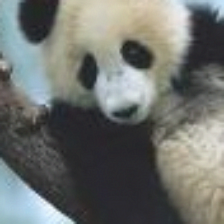
\includegraphics[width=.2\textwidth]{gibbon_993.png} \\
		$\centering \vec x$     &%
		& $\sgn \nabla_{\vec x} L(h(\vec x; \theta), y)$ & & $\widetilde{\vec x}$ \\
		\emph{panda} (0.577) & & & & \emph{gibon} (0.993) 
	\end{tabular}
	\caption{Prilagođeni prikaz dobivanja neprijateljskog primjera FGSM-om iz \cite{goodfellow14-ehae}. Nakošene riječi predstavljaju razrede, a brojevi u zagradama vjerojatnosti koje neuronska mreža dodjeljuje razredima.}
	\label{panda}
\end{figure}

\paragraph{Pronalaženje neprijateljskih primjera} Neka je $d:\mathcal{X}\times\mathcal{X}$ funkcija udaljenosti u ulaznom prostoru. Za svaki primjer $\vec x$ može se definirati susjedstvo $B_\epsilon(\vec x) = \{\widetilde{\vec x} : d(\widetilde{\vec x},\vec x)\leq\epsilon\}$. Pronalaženje neprijateljskih primjera se može definirati kao optimizacijski problem \cite{szegedy13-intrig-ipnn, cisse17-pn, madry17-tdlmraa} pronalaženja primjera $\widetilde{\vec x}$ koji maksimizira gubitak uz ograničenje da se nalazi u susjedstvu $B_\epsilon$ prirodnog primjera $\vec x$:
\begin{equation}
\widetilde{\vec x} = \argmax_{\widetilde{\vec x}\in B_\epsilon(\vec x)} L(h(\widetilde{\vec x}; \theta), y).
\end{equation}
Za funkciju udaljenosti $d$ se obično uzima neka $p$-norma razlike \cite{goodfellow14-ehae, cisse17-pn, madry17-tdlmraa}. Npr. za $\infty$-normu je $B_\epsilon(\vec x) = \{\widetilde{\vec x} : \lVert \widetilde{\vec x}-\vec x\rVert_\infty\leq\epsilon\}$.

Neprijateljski primjeri mogu se pronaći iterativnim optimizacijskim postupcima prvog reda uz održavanje ograničenja susjedstva. Pokazuje se da je neprijateljske primjere moguće pronaći već samo jednim korakom u smjeru predznaka gradijenta po svakoj dimenziji. Jedna vrsta takvog napada je "\emph{fast gradient sign method}" (FGSM) \cite{goodfellow14-ehae}. Neprijateljskom primjeru koji se pronalazi FGSM-om odgovara sljedeći izraz:
\begin{equation}
\widetilde{\vec x} = \vec x + \epsilon\sgn \nabla_{\vec x} L(h(\vec x; \theta), y).
\end{equation}
U \cite{madry17-tdlmraa} definiran je iterativni postupak koji se temelji na FGSM-u i autori ga nazivaju \emph{projected gradient descent} (PGD):
\begin{equation} \label{eq:pgd}
\widetilde{\vec x} \gets \Pi_{B_\epsilon(\vec x)} (\widetilde{\vec x} + \alpha\sgn\nabla_{\widetilde{\vec x}} L(h(\widetilde{\vec x}; \theta), y)).
\end{equation}
$\alpha$ je veličina koraka optimizacije, a $\Pi_{B_\epsilon(\vec x)}$ ovdje predstavlja projekciju na zatvorenu $\epsilon$-kuglu oko prirodnog primjera $\vec x$ uz $\infty$-normu. Npr. projekcijom vektora $\vec v$ na susjedstvo vektora $\vec x$, $\Pi_{B_\epsilon(\vec x)}(\vec v) = \argmin_{\vec v'\in B_\epsilon(\vec x)}\lVert \vec v'-\vec v\rVert_\infty$, svakoj komponenti $v_i$ dodjeljuje se najbliža vrijednost unutar intervala $\left[x_i-\epsilon, x_i+\epsilon\right]$.

Mogući su i napadi bez uvida u strukturu modela, npr. genetskim algoritmom. Također, pokazuje se da su neprijateljski primjeri u velikoj mjeri prenosivi između različitih modela \cite{szegedy13-intrig-ipnn, goodfellow14-ehae, liu-dtaeba}.

\paragraph{Neprijateljski rizik.} Može se definirati oblik rizika koji se može nazvati \emph{neprijateljskim rizikom} \cite{madry17-tdlmraa}:
\begin{equation}\label{eq:adv-risk}
\widetilde{R}(\vec\theta) = \widetilde{R}(\vec\theta;d,\epsilon) = \mathbb{E}_{(\vec x,y)\sim\mathcal{D}}\left[
\max_{\widetilde{\vec x} \in B_\epsilon(\vec x)} L(h(\widetilde{\vec x}; \theta), y) \right].
\end{equation}
Mali neprijateljski rizik predstavlja dobru lokalnu generalizaciju u susjedstvu prirodnih primjera.

\paragraph{Učenje s neprijateljskim primjerima} Trenutno najuspješniji pristup za postizanje otpornosti na neprijateljske primjere je učenje s neprijateljskim primjerima (engl. \emph{adversarial training}). Kod učenja s neprijateljskim primjerima skup za učenje se proširuje neprijateljskim primjerima koji se tijekom učenja prilagođavaju parametrima mreže \cite{goodfellow14-ehae, kurakin-amls}.

U nedavno objavljenom radu \cite{madry17-tdlmraa} eksperimentalno je pokazano da je učenjem s neprijateljskim primjerima dobivenim PGD-om (jednadžba~\ref{eq:pgd}) moguće postići dobru otpornost na neprijateljske primjere. Također, rezultati pokazuju da je za postizanje otpornosti na neprijateljske primjere uz održavanje dobre generalizacije potreban značajno veći kapacitet mreže.

\chapter{Parsevalove mreže}

U \cite{cisse17-pn} autori predstavljaju tzv. \emph{Parsevalove mreže}. Kod njih se kontrolira Lipschitzova konstanta svih slojeva i cijele mreže tako da ne bude veća od 1 i vrši se posebna vrsta regularizacije nad matricama težina. Motivacija je postizanje otpornosti na neprijateljske primjere kod dubokih neuronskih mreža. Kao najvažnija značajka Parsevalovih mreža ističe se to da se matrice težina linearnih i konvolucijskih slojeva ograničavaju tako da približno odgovaraju Parsevalovim uskim okvirima, tj. da budu ortogonalne matrice poopćene na nekvadratne matrice. Prema autorima, takve mreže postižu bolju otpornost na naprijateljske primjere generirane FGSM-om od odgovarajućih mreža koje nisu Parsevalove, brže se uče i njihov kapacitet se bolje iskorištava.

\section{Ograničavanje neprijateljskog rizika Lipschitzovom konstantom}

Lipschitzova konstanta funkcije $f$, ako postoji, definirana je ovako:
\begin{equation}
\Lambda = \sup_{\vec x\neq \widetilde{\vec x}} \frac{\lVert f(\vec x)-f(\widetilde{\vec x})\rVert}{\lVert \vec x-\widetilde{\vec x}\rVert}.
\end{equation}
Za funkcije za koje je Lipschitzova konstanta definirana kaže se da su Lipschitz-kontinuirane.

Klasifikator je funkcija $\hat{h}:\mathbb{R}^D\times{\varTheta} \to \mathcal{Y}$, gdje je $D$ dimenzija ulaznog prostora, $\Theta$ prostor parametara, a $\mathcal{Y}=\{0..C\}$ uz to da je $C$ broj razreda. Neuronske mreža za klasifikaciju su obično funkcije $h$ koje ulaz preslikavaju u vektor dimenzije $C$ koji predstavlja kategoričku razdiobu razreda i vrijedi $\hat{h}(\vec x;\vec\theta) = \argmax_y h(\vec x;\vec\theta)_y$. U daljnjem razmatranju mreža će se nekad predstavljati funkcijom $g$ kojoj su kodomena realni vektori koji predstavljaju kategoričke logite, tj. vrijedi $h(\vec x;\vec\theta) = \softmax(g(\vec x;\vec\theta))$.

Neuronska mreža se može prikazati kao usmjereni aciklički računski graf $G = (\mathcal{N}, \mathcal{E})$ gdje je svaki čvor $n\in\mathcal{N}$ funkcija svoje djece:
\begin{equation}
n(\vec x)=f^{(n)}(\vec\theta^{(n)}, (n'(\vec x))_{n':(n,n')\in\mathcal{E}}).
\end{equation}
Funkcija $h(\vec x) = h(\vec x;\vec\theta)$ koju ostvaruje mreža je korijen toga grafa. U nastavku će $n'\lessdot n$ označavati da je $n$ roditelj od $n'$, tj. $(n,n')\in\mathcal{E}$.

Za gubitak klasifikatora koji kao izlaz daje kategoričku razdiobu obično se koristi gubitak unakrsne entropije:
\begin{equation}
L(h(\vec x;\vec\theta), y) = -\ln h(\vec x;\vec\theta)_y
\end{equation}
Gubitak se preko funkcije $g$ može izraziti ovako:
\begin{equation}
L(h(\vec x;\vec\theta), y) = -g(\vec x;\vec\theta)_y + \ln \sum_{y'\in\mathcal{Y}}\exp g(\vec x;\vec\theta)_{y'}.
\end{equation}
Radi jednostavnijeg zapisa definiramo funkciju $\ell$ tako da uvijek vrijedi $\ell(g(\vec x;\vec\theta),y) = L(h(\vec x;\vec\theta),y)$. Možemo Uz zadanu $p$-normu pretpostaviti da postoji $\lambda_p$ takav da
\begin{equation}\label{eq:loss-lipschitz}
\forall \vec z, \vec z'\in \mathbb{R}^C,\, \forall y\in\mathcal{Y},\,
\lvert \ell(\vec z,y)-\ell(\vec z',y)\rvert 
\leq \lambda_p \lVert \vec z-\vec z'\rVert_p.
\end{equation}
Vrijedi $\pderiv{\ell(\vec z,y)}{z_{y'}} = -\llbracket y'=y \rrbracket + \softmax(\vec z)_{y'}$ i u najgorem slučaju se za $\pderiv{\ell(\vec z,y)}{\vec z}$ može dobiti vektor redak kojemu je jedan element $-1$, jedan $1$, a svi drugi $0$. Njegova $2$-norma je $\sqrt 2$, a $\infty$-norma $2$. Zato za odgovarajuće Lipschitzove konstante gubitka s obzirom na logite vrijedi $\lambda_2=\sqrt 2$ i $\lambda_\infty=2$.

Uz neku $p$-normu, neka je $\lambda_p$ Lipschitzova konstanta funkcije gubitka s obzirom na logite, a $\Lambda_p$ Lipschitzova konstanta funkcije $g(\vec x)$, tj. izlaza sloja logita s obzirom na ulaz mreže. Za svaki $p$ i $\epsilon > 0$  iz izraza~\ref{eq:loss-lipschitz} i definicije rizika $R(\vec\theta)$ i neprijateljskog rizika $\widetilde{R}(\vec\theta)=\widetilde{R}(\vec\theta,p,\epsilon)$ može se pokazati da vrijedi
\begin{align}
\widetilde{R}(\vec\theta) 
&\leq R(\vec\theta) + \mathbb{E}_{(\vec x,y)\sim\mathcal{D}}\left[
\max_{\widetilde{\vec x} \in B_\epsilon(\vec x)} 
\lvert \ell(z(\vec x;\vec\theta),y)-\ell(z(\vec x;\vec\theta),y) \rvert \right] \\
&\leq R(\vec\theta) + \epsilon\lambda_p\Lambda_p.
\end{align}
Budući da uvijek vrijedi $R(\vec\theta) \leq \widetilde{R}(\vec\theta)$, slijedi
\begin{equation}
0 \leq \widetilde{R}(\vec\theta)-R(\vec\theta) \leq \lambda_p\Lambda_p\epsilon.
\end{equation}

Može se vidjeti da smanjivanje Lipschitzove konstante samo po sebi nije dovoljno za poboljšanje otpornosti na neprijateljske primjere. Promjenom Lipschitzove konstante općenito se može utjecati i na $\widetilde{R}(\vec\theta)$ i na $R(\vec\theta)$. Npr. uvođenjem množenja logita s nekim skalarom $\alpha\in[0,1)$ prije primjene $\softmax$-a, tako da bude $h(\vec x) = \softmax(\alpha g(\vec x))$, smanjuje se Lipschitzova konstanta mreže i razlika $\widetilde{R}(\vec\theta)-R(\vec\theta)$ postaje manja, ali time se samo povećava entropija izlazne razdiobe i ne utječe se na rezultat klasifikacije $\argmax_yh(\vec x)_y$. U slučaju kada $\alpha=0$, dobiva se $\widetilde{R}(\vec\theta)=R(\vec\theta)$, ali izlazna razdioba vjerojatnosti $h(\vec x;\vec\theta)$ postaje uniformna. Ozbiljniji primjeri smanjivanja Lipschitzove konstante su $L_1$ i $L_2$ regularizacija za koje se isto pokazalo da nemaju značajan utjecaj na otpornost na neprijateljske primjere \cite{szegedy13-intrig-ipnn,goodfellow14-ehae}. 

Autori u članku o Parsevalovim mrežama iskazuju još jedan argument koji ima veze s kontroliranjem Lipschitzove konstante referencirajući \cite{xu-rg}, ali to neće biti obrađeno u ovom izvještaju.

\section{Lipschitzova konstanta neuronske mreže}

Uz definiranje $\Lambda_p^{(n,n')}$ kao Lipschitzove konstante čvora $n$ s obzirom na njemu ulazni čvor $n'$, može se pokazati da vrijedi
\begin{equation}
\Lambda_p^{(n)} = \sum_{n'\lessdot n}
\Lambda_p^{(n,n')}\Lambda_p^{(n')}.
\end{equation}
% TODO: derivacija

\paragraph{Sloj linearnog preslikavanja.} Kod linearnih slojeva kod kojih $n(\vec x)=\mat W^{(n)}n'(\vec x)$ Lipschitzova konstanta s obzirom na ulaz $n'(\vec x)$ odgovara matričnoj normi matrice parametara $\mat W^{(n)}$ pa je 
\begin{equation}
\Lambda_p^{(n)} \leq \lVert \mat W^{(n)}\rVert_p\Lambda_p^{(n')}.
\end{equation}
Za afine transformacije vrijedi isto jer pomak ne utječe na Lipschitzovu konstantu.

\paragraph{Konvolucijski sloj.} Razmatramo konvolucijski sloj s $d$ prostornih dimenzija i jednom dimenzijom značajki. Tada konvolucijska jezgra, kojoj su sve dimenzije jednake $k$ (radi jednostavnijeg zapisa) i koja na svakom položaju po prostornim dimenzijama ulaza računa jedan element izlaza na temelju ulaza sa semantičkom dimenzijom $H$, sadrži $k^dH$ elemenata. Konvolucijskom sloju koji daje izlaz sa semantičkom dimenzijom $D$ ima složenu jezgru koja se sastoji od $D$ takvih (pod)jezgri. Može se definirati operator razmatanja $U$ koji polje dimenzija $H\times a_1\times\dots\times a_d$ pretvara u matricu dimenzija $k^dH\times \prod_{i\in\{1..d\}}a_i$ tako da se za svaki položaj jezgre svi elementi koje ona pokriva kopiraju u jedan vektor stupac \cite{sharan-epdl}. Ako se svaka podjezgra razmota u vektor redak i cijela jezgra prikaže kao matrica $\mat W^{(n)}$ dimenzija $D\times k^dH$, onda se konvolucija $n(\vec x) = \tens w^{(n)}*_d n'(\vec x)$ može prikazati kao matrično množenje koje kao rezultat daje $\mat W^{(n)}U(n'(\vec x))$,
što je matrica dimenzija $D\times \prod_{i\in\{1..d\}}a_i$ koja se opet može prikazati kao polje dimenzija $D\times a_1\times\dots\times a_d$. Budući da je $U$ linearan operator koji svaki element ulaza kopira $k^d$ puta, vrijedi $\lVert U(n'(\vec x))-U(n'(\widetilde{\vec x}))\rVert_2^2 \leq k^d\lVert n'(\vec x)-n'(\widetilde{\vec x})\rVert_2^2$ i dobiva se
\begin{align} \label{eq:konv-lipschitz}
\Lambda_2^{(n)} &\leq k^{d/2} \lVert \mat W^{(n)}\rVert_2\Lambda_2^{(n')}, \\ \Lambda_\infty^{(n)} &\leq \lVert \mat W^{(n)}\rVert_\infty\Lambda_\infty^{(n')}.
\end{align}

\paragraph{Aktivacijski sloj.} Kod aktivacijskih slojeva Lipschitzova konstanta s obzirom na ulaz čvora odgovara Lipschitzovoj konstanti prijenosne funkcije $\lambda_p^{(n)}$ pa vrijedi
\begin{equation}
\Lambda_p^{(n)} \leq \lambda_p^{(n)}\Lambda_p^{(n')}.
\end{equation}

\paragraph{Linearna kombinacija izlaza različitih slojeva.} Kod slojeva linearne kombinacije vrijedi $n(\vec x) = \sum_{n'\lessdot n}\alpha^{(n,n')}n'(\vec x)$, gdje su $\alpha^{(n,n')}$ skalari. Za Lipschitzovu konstantu vrijedi
\begin{equation} \label{eq:linear-combination}
\Lambda_p^{(n)} \leq \sum_{n'\lessdot n}\alpha^{(n,n')}\Lambda_p^{(n')}.
\end{equation}
Poseban slučaj takvog čvora je čvor zbrajanja kakav se javlja kod preskočnih veza u rezidualnim mrežama \cite{he15-resnet}. Za takav čvor je
\begin{equation}
\Lambda_p^{(n)} \leq \sum_{n'\lessdot n}\Lambda_p^{(n')}.
\end{equation}

%\paragraph{Konkatenacija izlaza različitih slojeva.}
%TODO

\section{Parsevalove mreže}

Kako bi se osiguralo ograničenje Lipschitzove konstante kroz cijelu mrežu, autori predlažu održavanje redaka matrica težina ortonormalnima i zamjenu zbrojeva kod preskočnih veza konveksnim kombinacijama. Održavanje takvih ograničenja autori nazivaju \emph{Parsevalovom regularizacijom}.

\paragraph{Ortogonalnost matrica težina} Neka Za matricu težina\footnote{Radi usklađenosti s oznakama autora, transformacijska matrica se ovdje označava s $\mat W^\transpose$ umjesto s $\mat W$ i izlaz se računa kao $\vec y=\mat W^\transpose \vec x$.} $\mat W^\transpose \in\mathbb{R}^{D\times H}$ s ulaznom dimenzijom $H$ i izlaznom dimenzijom $D$ cilj je održavati ograničenje da su singularne vrijednosti blizu $1$, tj. ako $D<H$, da vrijedi $\mat W^\transpose \mat W \approx \mat I_D$. Takvoj matrici je lako odrediti vlastite vrijednosti i ograničiti spektralnu normu kao i operatorsku $\infty$-normu. Iz izraza~\ref{eq:konv-lipschitz} slijedi da je kod konvolucijskih slojeva matricu težina potrebno podijeliti s $k^2$ kako bi se održalo ograničenje Lipschitzove konstante, tj. da bude $\Lambda_2^{(n)}\leq\Lambda_2^{(n')}$. Kako bi se održavalo ograničanje ortogonalnosti, autori prvo za sve matrice težina $\mat W$ definiraju regularizacijski gubitak:
\begin{equation}
R_\beta(\mat W) = \frac{\beta}{2}\lVert \mat W^\transpose \mat W-\mat I\rVert_2^2
\end{equation}
i koriste postupak prvog reda kako bi se održavao blizu 0. Za gradijent tog gubitka po matrici težina vrijedi $\nabla_{\mat W} R_\beta(\mat W)=\beta(\mat W\mat W^\transpose-\mat I)\mat W$. U Parsevalovim mrežama se nakon svakog ažuriranja težina radi efikasnosti primjenjuje jedan korak gradijentnog spusta po ovom gubitku:
\begin{equation}
\mat W \gets (1+\beta)\mat W-\beta \mat W\mat W^\transpose \mat W. 
\end{equation}

\paragraph{Ograničenje konveksnosti linearne kombinacije} Kod Parsevalovih mreža slojevi koji obavljaju linearnu kombinaciju ulaznih čvorova, kao što je zbrajanje kod preskočnih veza, zamjenjuju se slojevima koji obavljaju konveksnu kombinaciju. Neka je $\vec a$ vektor koji sadrži sve koeficijente iz jednadžbe \eqref{eq:linear-combination}. Koeficijenti se ograničavaju se tako da vrijedi $\sum_i \alpha_i=1$ i $\forall i\, \alpha_i \in \left[0,1\right]$. Tako se osigurava da Lipschitzove konstanta sloja s obzirom na ulaz ne bude veća od najveće Lipschitzove konstante među ulaznim čvorovima. $\alpha$ su parametri koji se uče i ograničenje se ostvaruje projekcijom koeficijenata nakon svakog koraka gradijentnog spusta. Općeniti postupak objašnjen je u članku. U slučaju preskočnih veza zbroj se sastoji od dvaju pribrojnika i on se zamjenjuje konveksnom kombinacijom
$n(\vec x) = \alpha n'(\vec x) + (1-\alpha)n''(\vec x)$, gdje su $n'$ i $n''$ djeca čvora $n$. Ograničavanje koeficijenta je onda jednostavno: $\alpha\gets\min\{\max\{\alpha, 0\},1\}$.


\section{Rezultati}

Autori su eksperimentalno evaluirali postupak s rezidualnim mrežama \cite{he15-resnet,he16-resnet-imdrn,zagoruyko16-wrn} na skupovima podataka MNIST, CIFAR-10, CIFAR-100 i SVHN i s mrežama s potpuno povezanim slojevima na skupovima MNIST i CIFAR-10. Ovdje će samo biti kratko opisani rezultati analize rezidualne mreže WRN-28-10 \cite{zagoruyko16-wrn} i odgovarajuće Parsevalove mreže na skupu podataka CIFAR-10.

Konfiguracija mreža i hiperparametri prikazani su u tablici~\ref{tab:hiperparametri}. Korišten je isti postupak učenja i proširivanja podataka kao u \cite{zagoruyko16-wrn}. Razlika između Parsevalove mreže i obične mreže WRN-28-10 je u ograničavanju matrica težina i konveksnim kombinacijama umjesto zbrojeva kod preskočnih veza. Grupna normalizacija utječe na Lipschitzovu konstantu, ali autori Parsevalovih mreža nisu naveli jesu li mijenjali nešto u vezi nje.

Autori zaključuju da se kod Parsevalovih mreža poboljšava otpornost na neprijateljske primjere, ubrzava učenje i bolje iskorištva kapacitet mreže. U tablici~\ref{tab:adv-robustness} prikazane su točnosti klasifikacije neprijateljskih primjera mreže WRN-28-10 ovisno o skupu podataka i vrsti regularizacije. Omjer signala i šuma u decibelima u tablici je za ulaz $\vec x$ i njegov pomak $\vec \delta$ definiran ovako: $\mathrm{SNR}_\mathrm{dB}(\vec x, \vec{\delta}) = 20 \log_{10} \frac{\lVert \vec x\rVert_2}{\lVert\vec \delta\rVert_2}$.

\begin{table}[h!]
	\begin{center}
		\bgroup\footnotesize
		\begin{tabular}{|c|l|c|c|c|c|c|}
			\hline
			{\bf }
			& {\bf Model}
			& {\bf Bez šuma} & {\bf $\varepsilon\approx50$} & {\bf $\varepsilon\approx45$} & {\bf $\varepsilon\approx40$} & {\bf $\varepsilon\approx33$} \\
			\hline
			\multirow{6}{*}{\rotatebox{90}{CIFAR-10}}
			& Vanilla
			& 95.63         & 90.16         & 85.97         & 76.62         & 67.21      \\
			& Parseval(OC)
			& 95.82         & 91.85         & 88.56         & 78.79         & 61.38      \\
			& Parseval
			& \textbf{96.28}          & \textbf{93.03}         & \textbf{90.40}         & \textbf{81.76}         & \textbf{69.10}      \\
			\cline{2-7}
			\cline{2-7}
			& Vanilla
			& 95.49         & 91.17         & 88.90         & 86.75         & 84.87      \\
			& Parseval(OC)
			& 95.59         & 92.31         & 90.00         & \textbf{87.02}         & \textbf{85.23}      \\
			& Parseval
			& \textbf{96.08}          & \textbf{92.51}         & \textbf{90.05}         & 86.89         & 84.53      \\
			\hline\hline
			\multirow{6}{*}{\rotatebox{90}{CIFAR-100}}
			& Vanilla
			& 79.70         & 65.76         & 57.27         & 44.62         & 34.49      \\
			&Parseval(OC)
			& 81.07         & 70.33         & 63.78         & 49.97         & 32.99      \\
			& Parseval
			& \textbf{80.72}          & \textbf{72.43}         & \textbf{66.41}         & \textbf{55.41}         & \textbf{41.19}      \\
			\cline{2-7}
			\cline{2-7}
			& Vanilla
			& 79.23         & 67.06         & 62.53         & 56.71         & 51.78      \\
			& Parseval(OC)
			& \textbf{80.34}         & 69.27         & 62.93         & 53.21         & \textbf{52.60}      \\
			& Parseval
			& 80.19          & \textbf{73.41}         & \textbf{67.16}         & \textbf{58.86}         & 39.56      \\
			\hline\hline
			\multirow{3}{*}{\rotatebox{90}{SVHN}}
			& Vanilla
			& \textbf{98.38}        & 97.04        & 95.18        & 92.71        & 88.11     \\
			& Parseval(OC)
			& 97.91       & \textbf{97.55}        & \textbf{96.35}         & \textbf{93.73}         & \textbf{89.09}      \\
			& Parseval
			& 98.13        & 97.86        & 96.19         & 93.55         & 88.47      \\
			\cline{2-7}
			\hline
		\end{tabular}
		\egroup
	\end{center}
	\caption{
	Točnost klasifikacije mreže WRN-28-10 na skupovima CIFAR-10 i CIFAR-100 s različitim regularizacijama. $\varepsilon$ predstavlja omjer signala i šuma u decibelima. Za $\varepsilon=30$, čovjek može prepoznati da je dodan neprijateljski šum. Za svaki skup podataka prva 3 retka predstavljaju rezultate za učenje bez neprijateljskih primjera, a donja 3 retka za učenje s neprijatljskim primjerima. \emph{Parseval(OC)} označava mrežu na kojoj se ne koriste konveksne kombinacije, nego samo ograničenja ortogonalnosti. Tablica je preuzeta iz članka.
	}\label{tab:adv-robustness}
\end{table}

Na slici~\ref{fig:krivulje-pogreske} prikazane su krivulje učenja koje su dobili autori s Parsevalovom i neizmijenjenom rezidualnom mrežom na skupovima podataka CIFAR-10 i CIFAR-100.

\begin{figure}[htbp]
	\centering
	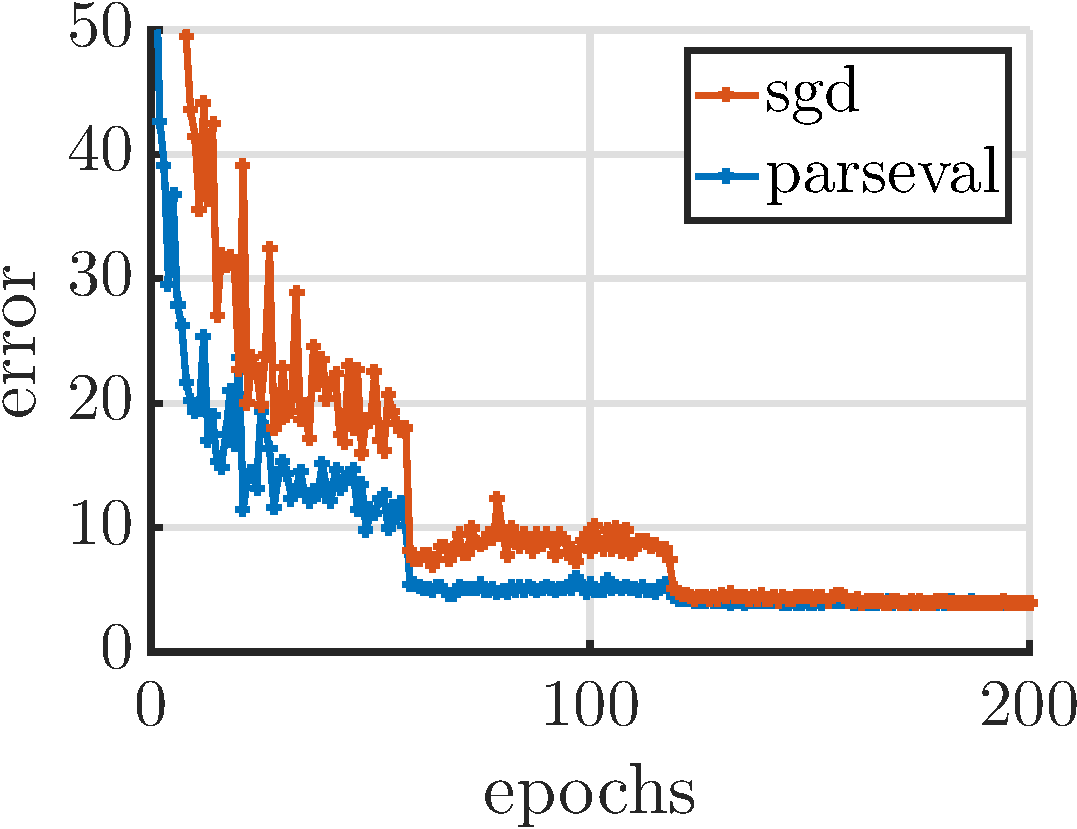
\includegraphics[width=0.49\linewidth]{ilustracije/convergence/cifar10.pdf}
	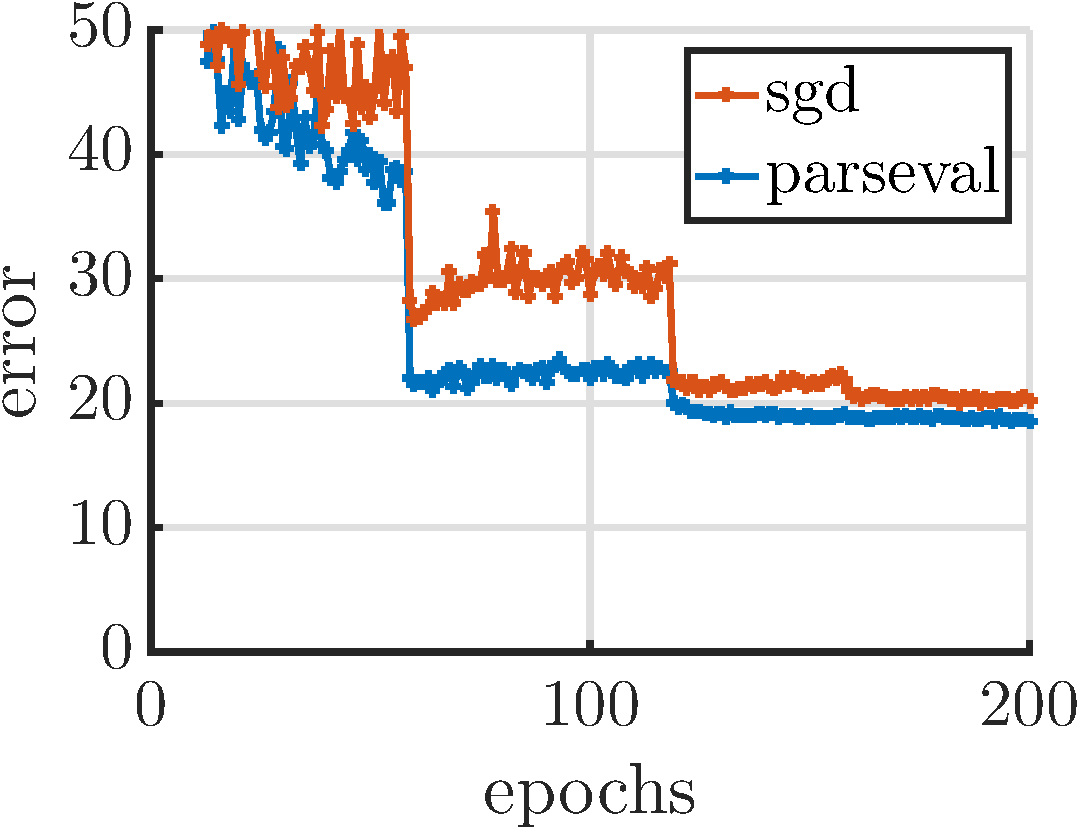
\includegraphics[width=0.49\linewidth]{ilustracije/convergence/cifar100.pdf}
	\caption{
		Krivulje koje pokazuju ovisnost klasifikacijske pogreške o broju završenih epoha koje su autori dobili učenjem obične (narančasto) i Parsevalove (plavo) mreže WRN-28-10 na skupovima CIFAR-10 (lijevo) i CIFAR-100 (desno). Slika je preuzeta iz članka.
	}
	\label{fig:krivulje-pogreske}
\end{figure}


\chapter{Programsko ostvarenje i rezultati} \label{chap:prog}

Autori Parsevalovih mreža \cite{cisse17-pn} nisu objavili izvorni kod i za projektni zadatak je bilo potrebno implementirati i evaluirati Parsevalovu rezidualnu mrežu. Pythonu je ostvarena biblioteka koja omogućuje definiranje općenite široke rezidualne mreže \cite{he15-resnet,he16-resnet-imdrn,zagoruyko16-wrn} u TensorFlow-u \cite{tensorflow2015-whitepaper}. Uz običnu rezidualnu mrežu implementirana je i odgovarajuća Parsevalova mreža. Izvorni kod je dostupan ovdje: \url{https://github.com/Ivan1248/Parseval-networks}.

Osim TensorFlowa, NumPyja, Matplotliba i drugih standardnih biblioteka korištena je i biblioteka CleverHans \cite{papernot2016cleverhans} za generiranje neprijateljskih primjera.

Za sve ekperimente je korištena rezidualna mreža koja bi trebala biti što sličnija mreži WRN-28-10 \cite{zagoruyko16-wrn} i njoj odgovarajuća Parsevalova mreža. Podskupovi skupa podataka CIFAR-10 korišteni su za učenje i evaluaciju.

\section{Razlike u odnosu na modele koje su autori koristili}

Ostvarene su rezidualne mreže koje bi trebale odgovarati Parsevalovoj i običnoj rezidualnoj mreži WRN-28-10. Poznate razlike u odnosu na modele koje su autori koristili su:
\begin{enumerate}
\item Za inicijalizaciju težina koristi se uniformna razdioba s varijancom $2/(k_1k_2H+D)$, dok su autori članka vjerojatno kao i \cite{zagoruyko16-wrn} koristili normalnu razdiobu s varijancom $2/k_1k_2H$, gdje su $k_1$ i $k_2$ prostorne dimenzije jezgre, $H$ semantička dimenzija ulaza, a $D$ semantička dimenzija izlaza konvolucijskog sloja.
\item Za grupnu normalizaciju se procjene očekivanja i varijance računaju kao eksponencijalni pokretni prosjek s ažuriranjem oblika $\hat{\mu}\gets0.95\hat{\mu}+0.05\mu_b$ koji se ažurira nakon svake mini-grupe $b$ tijekom učenja. Nije poznato koji su faktor autori koristili.
\item U blokovima u kojima se smanjuju prostorne, a povećava semantička dimenzija, preskočna veza zamjenjuje se sažimanjem usrednjavanjem po prostornim dimenzijama i dopunjavanjem nulama u semantičkoj dimenziji kao kod \cite{he15-resnet, he16-resnet-imdrn}. Kod \cite{zagoruyko16-wrn} se za to koristi konvolucija $1\times1$ s korakom $2$. U \cite{he16-resnet-imdrn} analizirane su neproširene rezidualne mreže i prema rezultatima se čini da dopunjavanje nulama daje malo bolje rezultate, ali nije poznato s koliko je značajna ta razlika.
\end{enumerate}
U članku ne piše kako su autori inicijalizirali koeficijente $\alpha$ slojeva konveksne kombinacije. Oni se ovdje inicijaliziraju brojem $0.99$. Bilo bi dobro analizirati utjecaj početnih vrijednosti koeficijenata $\alpha$ na učenje. Zasad se na temelju ne jako temeljitih eksperimenata čini da prije $20.$ epohe kod mreže WRN-28-1 razdioba koeficijenata kroz slojeve postane slična uniformnoj, ali malo koncentriranije oko početne vrijednosti. Primjer slučajnog uzorka naučenih koeficijenata je u tablici~\ref{tab:alfe}. %TODO ne???

Dobivene točnosti klasifikacije su otprilike $2$ postotna boda lošiji za obje mreže. Navedene razlike ne izgledaju kao da bi trebale imati značajan utjecati na točnost klasifikacije. Moguće je i da je negdje drugdje napravljena greška u implementaciji.


\section{Rezultati.} 

\paragraph{Brzina učenja i rezultati evaluacije} Na slici~\ref{fig:krivulje-pogreske-moje} su grafovi ovisnosti klasifikacijske pogreške o broju završenih epoha jednog mjerenja za Parsevalovu rezidualnu mrežu i jednog za običnu rezidualnu mrežu WRN-28-10 na podskupu za testiranje skupa CIFAR-10. Krivulje su konvergirale na točnost oko $0.94$. Stopa učenja je do $60.$ epohe $0.1$, a nakon $60.$, $120.$ i $160.$ se smanjuje množenjem s $0.2$. Glavni uzrok velikih oscilacija krivulja kod početne velike stope učenja je vjerojatno sporo ažuriranje pokretnog prosjeka statistika grupne normalizacije u odnosu na brzinu promjene parametara. 

\begin{figure}[htbp]
	\centering
	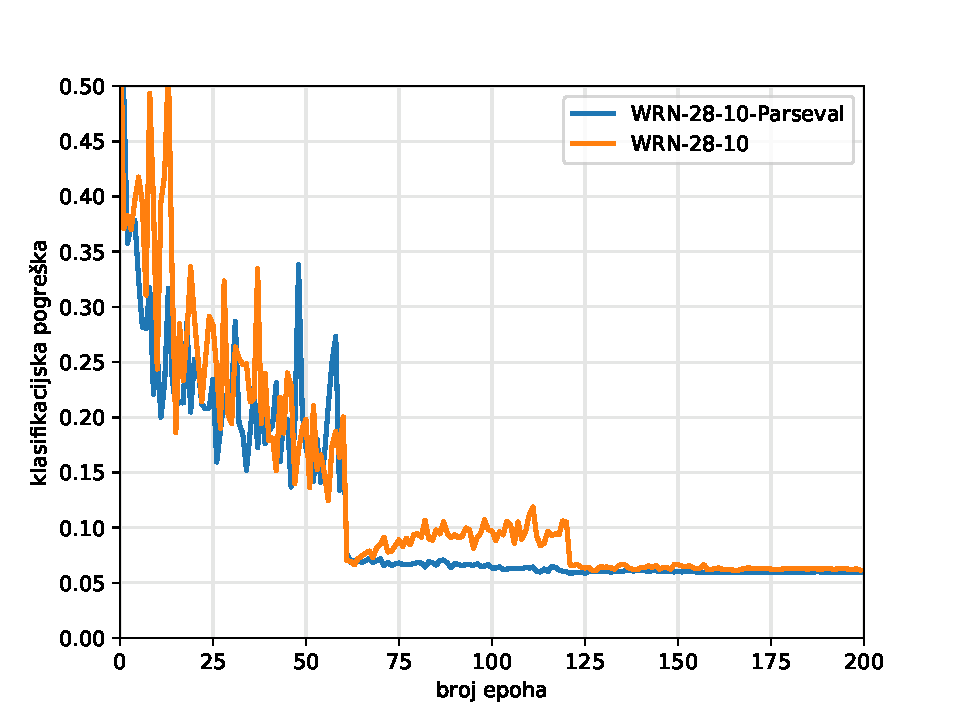
\includegraphics[width=1\linewidth]{ilustracije/grafovi/krivulje-pogreske}
	\caption{
		Ovisnost klasifikacijske pogreške o broju završenih epoha za Parsevalovu (plavo) i običnu (narančasto) rezidualnu mrežu. Svaka mreža se učila na uniji skupa za učenje i skupa za validaciju, a evaluirala na skupu za testiranje. Svaka krivulja je rezultat jednog mjerenja.
	}
	\label{fig:krivulje-pogreske-moje}
\end{figure}

\paragraph{Otpornost na neprijateljske primjere} Na slici~\ref{fig:krivulje-otpornosti} prikazane su krivulje koje pokazuju otpornost modela na neprijateljske primjere ovisno o $\infty$-normi pomaka dobivenog FGSM-om. Na slici~\ref{fig:neprijateljski-primjeri} su prikazani primjeri neprijateljskih primjera dobivenih za različite $\epsilon$.

\begin{figure}[htbp]
	\centering
	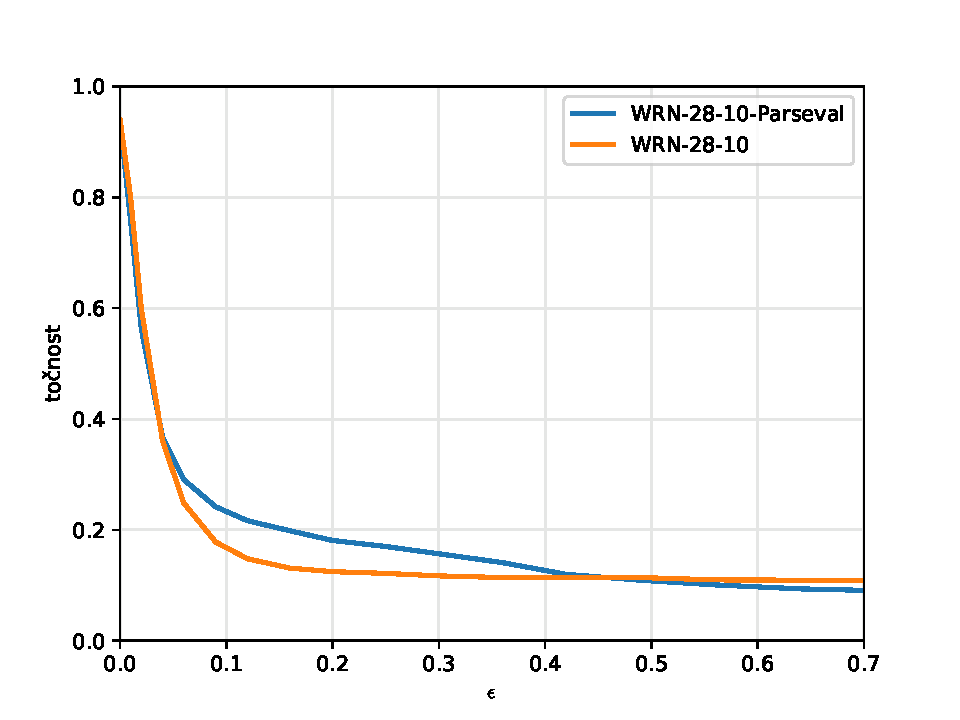
\includegraphics[width=1\linewidth]{ilustracije/grafovi/otpornost}
	\caption{
		Krivulje ovisnosti točnosti o iznosu $\infty$-norme šuma generiranog algoritmom FGSM za mreže iz slike~\ref{fig:krivulje-pogreske-moje}. Šum se dodaje normaliziranim slikama is podskupa za testiranje skupa CIFAR-10. Za dobivanje grafa su radi bržeg generiranja neprijateljskih primjera i evaluacije korištene 16384 slike iz skupa za testiranje.
	}
	\label{fig:krivulje-otpornosti}
\end{figure}

\begin{figure}[htbp]
	\centering
	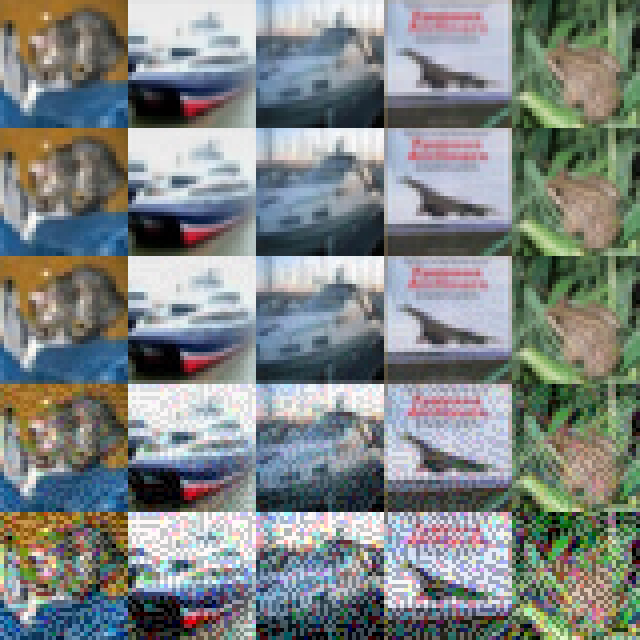
\includegraphics[width=0.6\linewidth]{ilustracije/slike/np-eps025251}
	\caption{
		Neprijateljski primjeri dobiveni FGSM-om za $\epsilon=0,0.02,0.05,0.2,0.5,1$ redom odozgo prema dolje.
	}
	\label{fig:neprijateljski-primjeri}
\end{figure}

\bibliography{literatura}
\bibliographystyle{fer}

\nocite{colah}
\nocite{nndl}



\appendix

\chapter{Konfiguracija rezidualnih mreža} \label{chap:hiperparametri}

\begin{table}[!htp] \centering
	\newcolumntype{L}[1]{>{\raggedright\let\newline\\\arraybackslash\hspace{0pt}}m{#1}}
	\resizebox{\textwidth}{!}{%
		\begin{tabular}{| L{\dimexpr 0.4\linewidth-2\tabcolsep} |
				L{\dimexpr 0.45\linewidth-2\tabcolsep} |
				L{\dimexpr 0.55\linewidth-2\tabcolsep} |}
			\hline
			\bf Ime hiperparametra & \bf Vrijednost & \bf Komentar  \\\hline
			\multicolumn{3}{|l|}{\bf Konvolucijski sloj}  \\\hline
			inicijalizacija težina 
				& $U(-M, M)$, $M=\sqrt{\frac{6}{k_0 k_1 H + D}}$ 
				& $k_0$ i $k_1$ su prostorne dimenzije jezgre, $H$ semantička dimenzija ulaza, a $D$ semantička dimenzija izlaza \\\hline
			inicijalna vrijednost pomaka & $\vec{0.05}$ & \\\hline
			\multicolumn{3}{|l|}{\bf Grupna normalizacija}  \\\hline
			stopa eksp. pokr. prosjeka & $0.95$ & 			\\\hline
			inicijalni pomak & $\vec 0$ & 	    \\\hline
			inicijalno skaliranje & $\vec 1$ & \\\hline
			\multicolumn{3}{|l|}{\bf Konveksna kombinacija (Parsevalova mreža)}  \\\hline
			koeficijent $\alpha$ & $0.99$ & $(\vec x, \vec r) \mapsto \alpha \vec x + (1-\alpha)\vec r$, $\alpha \in \left[0,1\right]$   \\\hline
			\multicolumn{3}{|l|}{\bf Rezidualni blok}  \\\hline
			broj konvolucijskih slojeva & $2$ & \\\hline
			prostorne dimenzije jezgri & $3$ & \\\hline
			dropout & $0.3$ & \\\hline
			način povećanja broja značajki & identitet s nadopunjavanjem nulama & \\\hline
			faktor proširenja $k$ \cite{zagoruyko16-wrn} & $10$ & (semantička dimenzija blokova prve grupe je $16k$) \\\hline
			\multicolumn{3}{|l|}{\bf Rezidualna mreža}  \\\hline
			duljine grupa & $(4,4,4)$ & (3 grupe s po 4 bloka)\\\hline
			$L_2$ regularizacija & $5\cdot 10^{-4}$ & \\\hline
			stopa učenja & $0.1$ na početku, u $60.$, $120.$ i $160.$ epohi se smanjuje množenjem s $0.2$ & \\\hline
			veličina mini-grupe & $128$ & \\\hline
			\multicolumn{3}{|l|}{\bf Rezidualna mreža (Parsevalova mreža)}  \\\hline
			$\beta$ (od $R_{\beta}$) & $10^{-4}$ & \\\hline
		\end{tabular}
	} % TODO: koristiti pmatrix za matrice i vektore
	\caption{Hiperparametri testiranih rezidualnih mreža.}
	\label{tab:hiperparametri}
\end{table}

\chapter{Ostali rezultati} \label{chap:hiperparametri}

\begin{table}[!htp] \centering
		\bgroup\footnotesize
		\begin{tabular}{|l|c|}
			\hline
			Blok & $\alpha$ \\
			\hline
			g0/b0 & 0.532 \\  
			g0/b1 & 0.708 \\ 
			g0/b2 & 0.704 \\ 
			g0/b3 & 0.713 \\ 
			g1/b0 & 0.272 \\ 
			g1/b1 & 0.481 \\ 
			g1/b2 & 0.771 \\ 
			g1/b3 & 0.682 \\ 
			g2/b0 & 0.203 \\ 
			g2/b1 & 0.418 \\ 
			g2/b3 & 0.012 \\ 
			g2/b2 & 0.286 \\ 
			\hline
		\end{tabular}
		\egroup
	\caption{Slučajan uzorak koeficijenata slojeva konveksne kombinacije nakon oko 22 epohe kod mreže WRN-28-1 uz početne vrijednosti $0.99$. "g$x$/b$y$" označava $y$-ti blok $x$-te grupe. }
	\label{tab:alfe}
\end{table}

\end{document}
